%% LyX 1.5.2 created this file.  For more info, see http://www.lyx.org/.
%% Do not edit unless you really know what you are doing.
\documentclass[english]{bioinfo}
\usepackage[latin1]{inputenc}
\usepackage{subfigure}
\setcounter{secnumdepth}{3}
\setcounter{tocdepth}{3}
\usepackage{esint}
\IfFileExists{url.sty}{\usepackage{url}}
                      {\newcommand{\url}{\texttt}}

\makeatletter
%%%%%%%%%%%%%%%%%%%%%%%%%%%%%% Textclass specific LaTeX commands.
 \usepackage{amsmath}
 \usepackage{amsfonts}
 \usepackage{natbib}
 \usepackage{ae}
\usepackage{bm}

%%%%%%%%%%%%%%%%%%%%%%%%%%%%%% User specified LaTeX commands.
\usepackage{crop}
\copyrightyear{2008}
\pubyear{2008}

\usepackage{babel}
\makeatother

\begin{document}
\selectlanguage{english}
\firstpage{1}

\title {Gaussian Process Modelling of Latent Chemical
  Species: Applications to Inferring Transcription Factor Activities}

\author {Pei Gao\,$^{1}$, Antti Honkela\,$^{2}$, Magnus Rattray\,$^{1}$
and Neil D. Lawrence\,$^{1,*}$%
\thanks {to whom correspondence should be addressed} }

\address {$^{1}$School of Computer Science, University of Manchester, Kilburn Building, Oxford Road, Manchester, M13 9PL\\
$^{2}$Adaptive Informatics Research Centre, Helsinki University of Technology, P.O. Box 5400, FI-02015 TKK, Finland}
\history {Received on XXXXX; revised on XXXXX; accepted on XXXXX}

\editor {Associate Editor: XXXXXXX}
\maketitle

\begin{abstract}

\section{Motivation:} Inference of \emph{latent chemical species} in biochemical interaction
networks is a key problem in estimation of the structure and
parameters of the genetic, metabolic and protein interaction networks
that underpin all biological processes. We present a framework for
Bayesian marginalisation of these latent chemical species through
Gaussian process priors.

\section{Results:} We demonstrate our general approach on three different biological examples
of single input motifs, including both activation and repression of
transcription.  We focus in particular on the problem of inferring
transcription factor activity when the concentration of active protein
cannot easily be measured. We show how the uncertainty in the inferred
transcription factor activity can be integrated out in order to derive
a likelihood function that can be used for the estimation of
regulatory model parameters.  An advantage of our approach is that we
avoid the use of a coarse-grained discretization of continuous-time
functions, which would lead to a large number of additional parameters
to be estimated. We develop efficient exact and approximate inference
schemes, which are much more efficient than competing sampling-based
schemes and therefore provide us with a practical toolkit for
model-based inference.

\section{Availability:} The software and data for recreating all the experiments in this paper
is available in MATLAB from \url{http://www.cs.man.ac.uk/~neill/gpsim} 

\section{Contact:} \url{neill@cs.man.ac.uk}
\end{abstract}

\section{Introduction}

Ordinary differential equations (ODEs) are the most common framework
in use for modelling biological
sub-systems~\citep{Alon:systems06}. Well established methodologies
have been developed for estimating the parameters of these equations
in the context of a particular experiment or set of experiments, using
\emph{e.g.} least squares and maximum likelihood combined with an
appropriate optimisation algorithm~\citep{MendesKell98}. More
recently, significant progress has been made on Bayesian parameter
estimation in the context of ODEs (\emph{e.g.}
\citealp{Coleman06}). Through the use of advanced Monte Carlo
techniques it is even possible to, given a specific data set, rank
model structures through the use of Bayes factors
\citep{Vyshemirsky:ranking08}. This shows the potential for ODE models
to be closely integrated with biological investigations, informing the
process of biological experimental design.

A challenging problem for differential equation modelling occurs where
one or more chemical species influencing the dynamics are controlled
outside of the sub-system being modelled. For example, a signalling
pathway can be triggered by a signal external to the pathway
itself. In a regulatory sub-system, one or more transcription factors
(TFs) may influence the expression of a set of target genes, but these
TFs may not be regulated at the transcriptional level, instead being
activated by another sub-system such as a signalling
pathway. Similarly, in a metabolic pathway external metabolites and
enzymes will influence the dynamics of the pathway. If these external
chemical species have a constant influence, \emph{e.g.} as in the case
of steady-state behaviour of a metabolic pathway, then they can simply
be treated as additional parameters of the model and their effect can
be estimated along with the other model parameters. However, more
often these external factors are time-varying quantities. In this case
they are functional parameters and cannot be estimated by the standard
methods discussed above. One approach for dealing with this is to
discretize in time, treating the time varying function as a sequence
of discrete parameters. However, this leaves the problem of choosing
the correct granularity for the discretization and either ignoring
temporal continuity, or assuming a simple Markovian relationship and
thereby introducing further model parameters and assumptions. Here we
propose an alternative approach. We deal with these parameters as
continuous functions of time, avoiding the need for arbitrary
discretisation.

To further compound the problem of dealing with the time-varying
effects of these chemical species, their concentration is often not
directly observable and their dynamics must therefore be inferred
indirectly according to their influence on measured elements of the
system. This is a common problem and it is a natural consequence of
the fact that some quantities are relatively easy to measure in a high
throughput manner (\emph{e.g.} mRNA concentrations with a microarray),
whereas others are much more difficult to measure (\emph{e.g.}  the
concentration of transcription factors located in the nucleus). In
this paper we advocate the use of Gaussian processes to define prior
distributions over these \emph{latent chemical species}. This allows
us to marginalise their contributions in the interaction network of
interest. We present a basic toolkit of algorithms based on Gaussian
processes which allow us to consider different response models
(Michaelis Menten kinetics, repression responses) and cascades of
interactions in which chemical species of interest are missing. The
application domain we consider is inference of transcription factor
(TF) activity in both developmental and signalling networks.

Inference of TF activity in a given network is a well studied problem
with both genome wide approaches (\emph{e.g.}
\citealp{Liao:nca03,Sanguinetti:chipdyno06,Sanguinetti:chipvar06}) and
algorithms designed for a sub set of genes (\emph{e.g.}
\citealp{Nachman:inferring04,Rogers:model06b,Khanin:repression06,Barenco:ranked06}). Our
approach is most directly inspired by \cite{Barenco:ranked06} who
infer transcription factor activity in a single input module network
motif through a differential equation with a linear response. We build
on their work to consider simple cascade networks and non-linear
response models such as Michaelis Menten kinetics and repression
responses (\citealp{Alon:systems06,Khanin:repression06}).

Gaussian processes \citep{Rasmussen:book06} are probabilistic models
of functions that encode particular assumptions about the function
such as smoothness and timescale. They are commonly applied in the
context of regression and interpolation. An attractive characteristic
of the Gaussian process (GP) is that the result of any linear operator
on the function leads to another GP and we will exploit this when
applying GPs in the context of differential equations.

Our focus in this paper will be the inference of transcription factor
activities given mRNA concentrations. We start by considering the
model given in \cite{Barenco:ranked06} and reviewing the work done by
\cite{Lawrence:transcriptionalGP06} who provided the first treatment
of this model with GPs. Then, in Section~\ref{sub:repressionModel}, we
extend our model to the case of repression. We follow
\cite{Khanin:repression06} and apply the model in the context of the
SOS system in {\em E. coli} where genes are controlled by the
transcriptional repressor protein LexA. In both these cases, no model
of transcription factor translation is included as the proteins are
post-translationally regulated. In our final example
(Section~\ref{sub:cascadedDifferentialEquations}) we show how, in the
context of \emph{Drosophila} mesoderm development, a model of
translation can also be incorporated to improve the quality of the
transcription factor inference in cases where TFs are primarily
regulated at the transcriptional level.

\section{Methods and Results}

The following linear model of gene activation was considered by
\cite{Barenco:ranked06},
\begin{equation}
\frac{\mathrm{d}x_{j}\left(t\right)}{\mathrm{d}t}=B_{j}+S_{j}f\left(t\right)-D_{j}x_{j}\left(t\right),
\label{eqn:linearModel}
\end{equation}
where the changing level of a gene $j$'s expression,
$x_{j}\left(t\right)$, is given by a combination of a basal
transctiption rate, $B_{j}$, a sensitivity, $S_{j}$, to its governing
TF's activity, $f\left(t\right)$, and the decay rate of the mRNA,
$D_{j}$. The differential equation can be solved for
$x_{j}\left(t\right)$ giving
%
\begin{equation}
x_{j}\left(t\right)=\frac{B_{j}}{D_{j}}+S_{j}\int_{0}^{t}e^{-D_{j}\left(t-u\right)}f\left(u\right)\mathrm{d}u,\label{eq:linearSolution}
\end{equation}
%
where we have ignored any transient terms (we can assume these are
zero if the TF has zero concentration at times before $t=0$).

\begin{figure*}[t]
\centering
\subfigure[]{
	\label{fig:activation:a}
	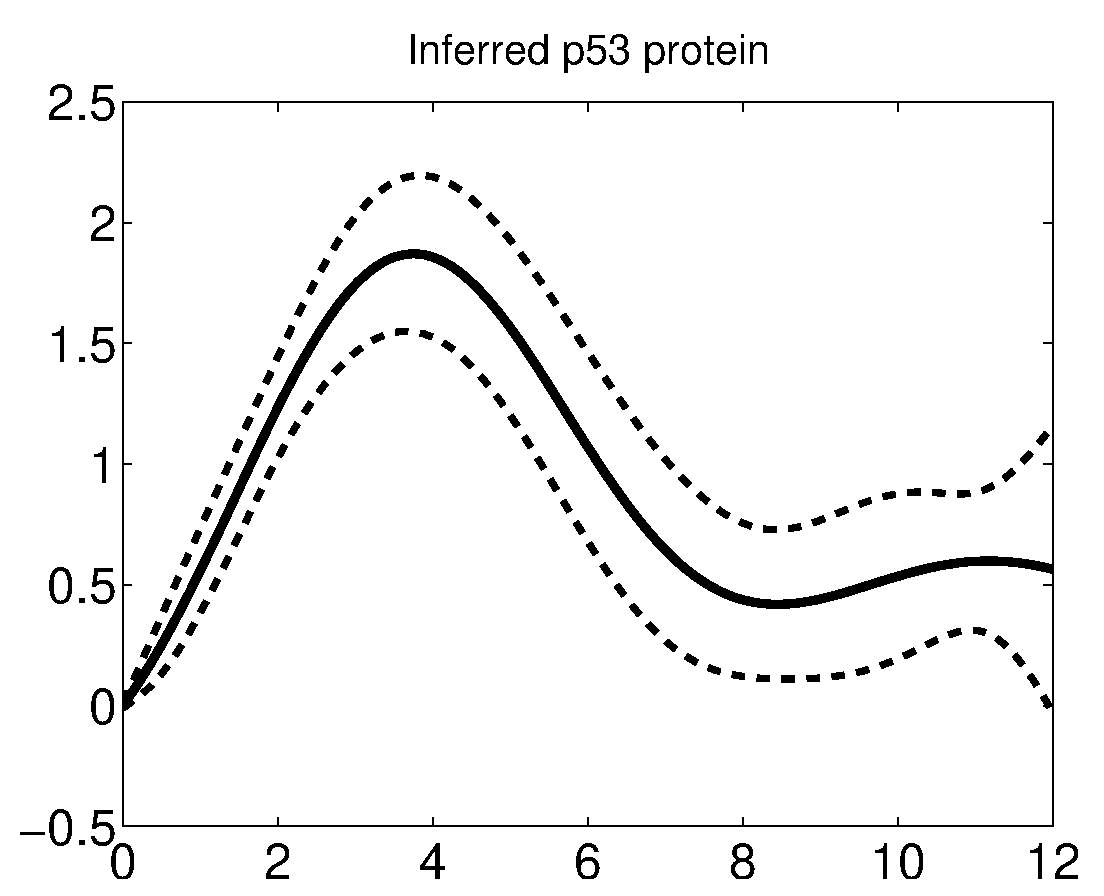
\includegraphics [height=1.6in, width=0.3\textwidth] {./diagrams/demBarenco1_profile2.eps} }
\subfigure[]{
	\label{fig:activation:b} 
	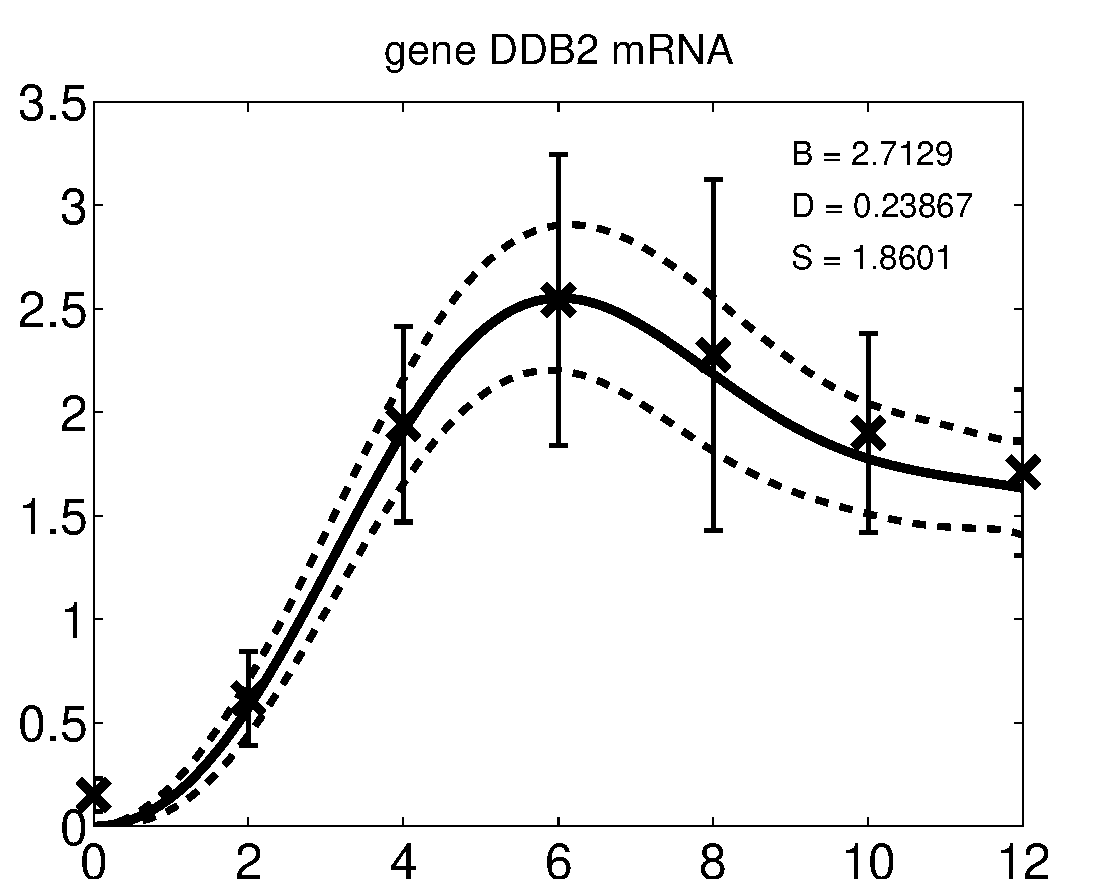
\includegraphics [height=1.6in, width=0.3\textwidth]{./diagrams/demBarenco1_ExprsProfile_Rep2_Gene1.eps} }
\subfigure[]{
	\label{fig:activation:c}
	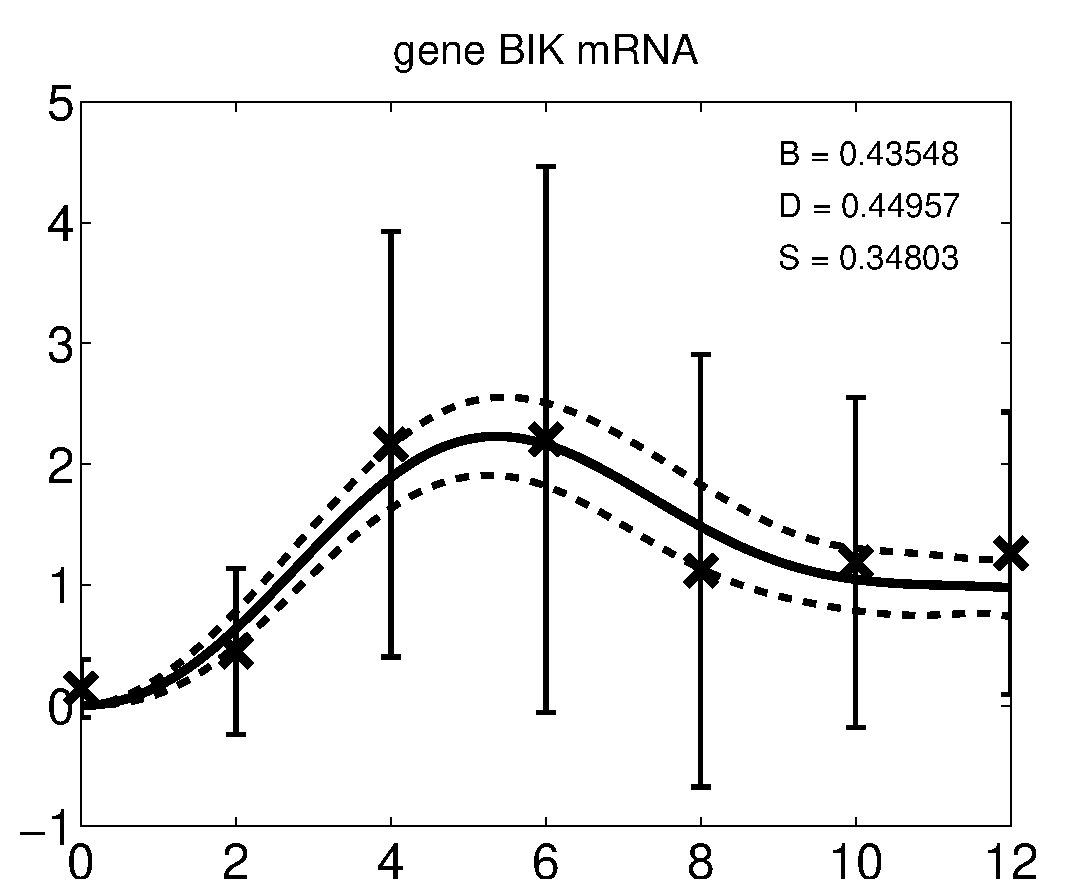
\includegraphics [height=1.6in, width=0.3\textwidth]{./diagrams/demBarenco1_ExprsProfile_Rep2_Gene2.eps} }
\subfigure[]{
	\label{fig:activation:d}
	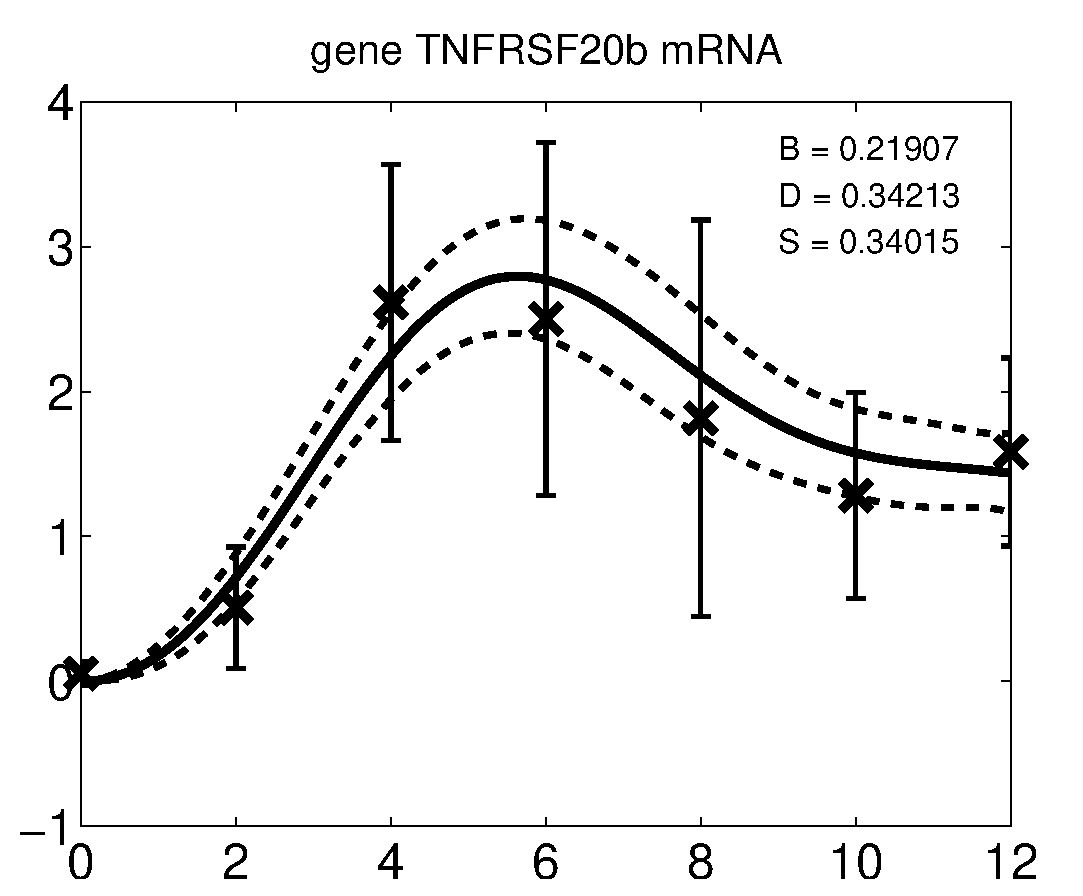
\includegraphics [height=1.6in, width=0.3\textwidth]{./diagrams/demBarenco1_ExprsProfile_Rep2_Gene3.eps} }
\subfigure[]{
	\label{fig:activation:e}
	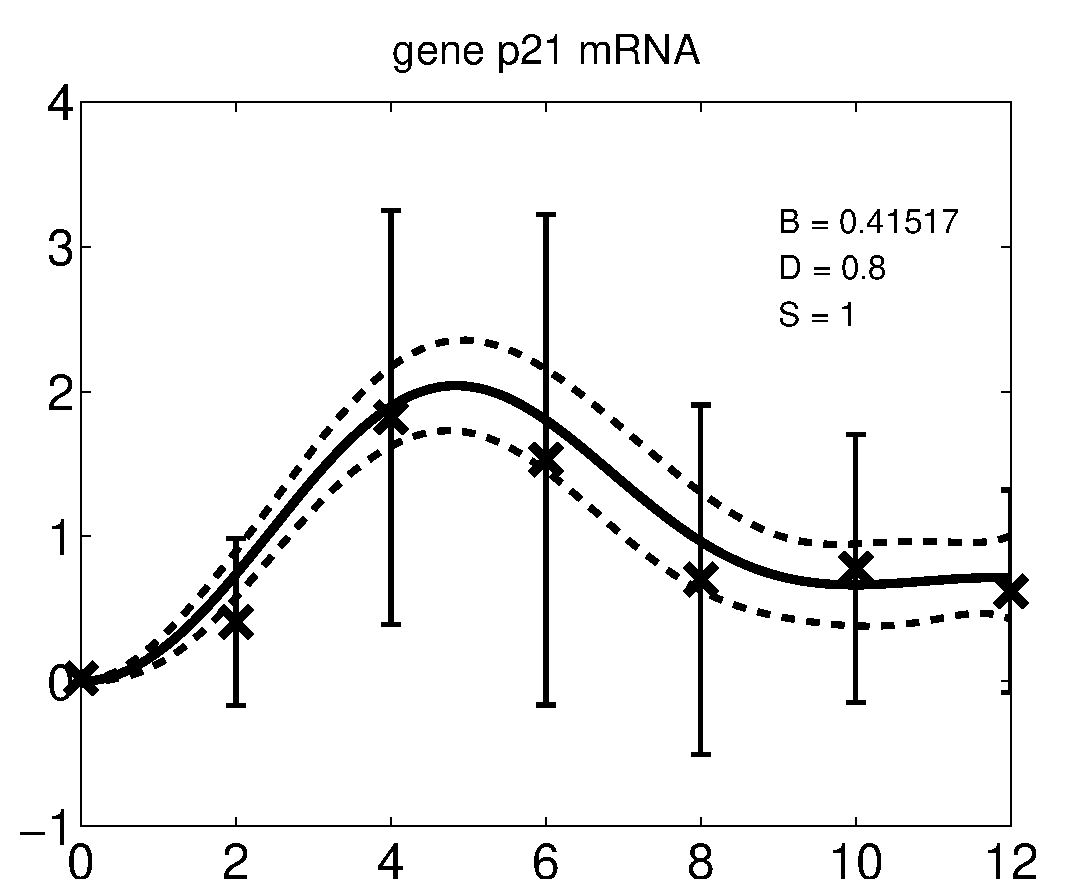
\includegraphics [height=1.6in, width=0.3\textwidth] {./diagrams/demBarenco1_ExprsProfile_Rep2_Gene4.eps} }
\subfigure[]{
	\label{fig:activation:f}
	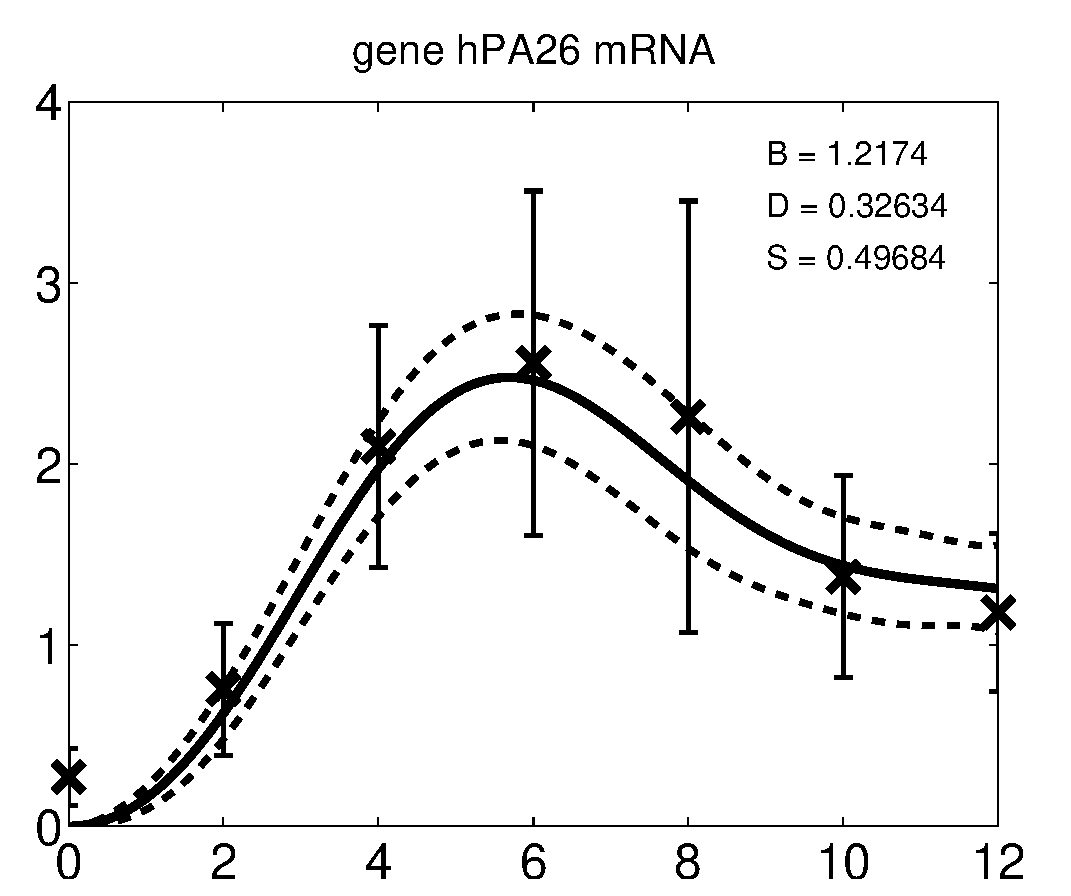
\includegraphics [height=1.6in, width=0.3\textwidth] {./diagrams/demBarenco1_ExprsProfile_Rep2_Gene5.eps}
}
\caption{Results for p53 using the linear model and a GP with RBF
  kernel. Results are shown for one replicate: (a) predicted protein
  concentration; (b) predicted expression level for DDB2; (c)
  predicted expression level for BIK; (d) predicted expression level
  for TNFRSP20b; (e) predicted expression level for p21; (f) predicted
  expression level for hPA26. Solid lines represent the mean
  inference, dashed lines are 95\% credibility intervals, and the
  crosses are the observed gene expression data with error bars
  showing the technical error from each individual Affymetrix
  microarray~\citep{Liu05}. Maximum likelihood model parameters,
  estimated using all replicates, are shown for each target
  gene.} \label{fig:activation}
\end{figure*}

\subsection{Gaussian process inference}
\label{sec:gp}

Our general approach is to assume that $f\left(t\right)$ was drawn
from a Gaussian process. A Gaussian Process (GP) is a prior
distribution over functions that leads to highly flexible non-linear
functions in which characteristics such as the stationarity, the
roughness and the timescale of the signal can be controlled. GPs are
the functional analogue of the Gaussian distribution, they are fully
specified by a mean function, $\mu\left(t\right)$, and a covariance
function, $k\left(t,t^{\prime}\right)$. The mean function is an
unconstrained function of time, whilst the covariance function is
constrained to be a positive definite function. Various covariance
functions can be used but we will predominantly make use of the
squared exponential covariance (sometimes known as the Gaussian or RBF
covariance),
%
\begin{equation}
k\left(t,t^{\prime}\right)=\exp\left(-\frac{\left(t-t^{\prime}\right)^{2}}{l^{2}}\right)
\ .
\label{eqn:squaredExp}
\end{equation}
%
An important characteristic of a GP is that any linear operation
applied to the function drawn from a GP leads to a function that is
drawn from a related GP. This is the functional analogue of linear
operations applied to samples from a Gaussian distribution. We note
that (\ref{eq:linearSolution}) is a linear operation on
$f\left(t\right)$ since the integral is the functional analogue of a
weighted sum. The properties of the GP tell us that if
$f\left(t\right)$ was drawn from a GP with covariance function
$k_{f,f}\left(t,t^{\prime}\right)$ then $x_{j}\left(t\right)$ will
also be drawn from a GP with a covariance function given by
\begin{equation}
k_{x_{j},x_{j}}\left(t,t^{\prime}\right)=S_{j}^{2}\int_{0}^{t}\int_{0}^{t^{\prime}}\mathrm{e}^{-D_{j}\left(t-u+t^{\prime}-u^{\prime}\right)}k_{f,f}\left(t,t^{\prime}\right)\mathrm{d}u\mathrm{d}u^{\prime}
\ .
\label{eqn:kxjxj}
\end{equation}
Furthermore, the cross covariances between the $x_{j}\left(t\right)$
and $f\left(t\right)$ will be given by
\begin{equation}
k_{x_{j},f}\left(t,t^{\prime}\right)=\int_{0}^{t}e^{-D_{i}\left(t-u\right)}k_{f,f}\left(t,t^{\prime}\right)\mathrm{d}u
\ .
\label{eqn:kxjf}
\end{equation}
Finally, if our data consist of several genes, $\left\{
x_{j}\left(t\right)\right\} _{j=1}^{N}$, cross covariances between the
genes can be computed,
\begin{equation}
k_{x_{i},x_{j}}\left(t,t^{\prime}\right)=S_{i}S_{j}\int_{0}^{t}\!\int_{0}^{t^{\prime}}\!\!\!\!e^{-D_{i}\left(t-u\right)-D_j\left(t^{\prime}-u^{\prime}\right)}k_{f,f}\left(t,t^{\prime}\right)\mathrm{d}u\mathrm{d}u^{\prime}
\ .
\label{eqn:kxixj}
\end{equation}
The basal transcription rate then appears in the mean function to
define the mean of the Gaussian process for $x_{j}\left(t\right)$ as a
constant $B_{j}/D_{j}$.

As was shown in \cite{Lawrence:transcriptionalGP06}, if
$f\left(t\right)$ is drawn from a GP with a squared exponential
covariance function, we can analytically define a probabilistic model
of the expression data for which the parameters of the differential
equation, $B_{j},\, S_{j},\, D_{j}$ and the timescale $l$ can all be
determined, either through maximum likelihood or Bayesian sampling.

A likelihood function for the model parameters $\theta=\{B_{j},\,
S_{j},\, D_{j}\}_{j=1}^N$ and GP length scale $l$ is obtained by {\em
  integrating out} the latent function $f(t)$
\begin{equation}
L(\theta,l) = \int \left(\prod_{j} p(\bm x_j|\theta,f(t))\right)
p(f(t)|l) \, \mathrm{d}f(t) \ , 
\label{eqn:likelihood}
\end{equation}
where the data $\bm x_j = [x_j(t_i)]$ are collected at discrete times
$t_i$ and modelled using Gaussian observation noise with either known
or estimated variance (this is for a single replicate). Integrating
out $f(t)$ avoids having to carry out maximum likelihood for this
infinite dimensional parameter which could be problematic as estimates
based on limited data would be associated with large
uncertainty. Approaches based on carrying out maximum likelihood over
a discretized $f(t)$ suffer from the same problem, \emph{i.e.} the
discretisation introduces many new parameters which have to be
estimated and therefore only a very coarse discretization will be
tractable~\citep{Khanin:repression06}. The associated error in these
parameters confounds the estimation of other parameters by maximum
liklihood and while Bayesian approaches avoid this problem there is a
large associated computational bottleneck in using Markov chain Monte
Carlo (MCMC) on these extra
parameters~\citep{Rogers:model06b,Barenco:ranked06}.

We illustrate our results from applying the method below, first on the
previously studied linear activation model and then showing how we can
extend the approach to non-linear response functions for activation
and repression, followed by a two-layer activation model.

\subsection{Activation}

In this section we consider a system in which a single TF activates a
number of targets. The example we consider is the TF p53 which is a
tumour repressor activated during DNA damage. According to
\citet{Barenco:ranked06}, irradiation is performed to disrupt the
equilibrium of the p53 network and the transcription of p53 target
genes are then stimulated. Seven samples of the expression levels of
the target genes in three replicas are collected as the raw time
course data.

\subsubsection{Linear Activation}

In this section we recreate the results presented by
\citet{Lawrence:transcriptionalGP06} for the linear model with several
key differences. Firstly, in their original paper
\citet{Barenco:ranked06} constrained $f\left(0\right)$ to be zero,
forcing the basal transcription rate to account for all transcription
at time $t=0$. This constraint was not included in
\citeauthor{Lawrence:transcriptionalGP06} but is included here. This
allows us to incorporate the prior information of the latent TF
profiles as much as possible. Secondly,
\citeauthor{Lawrence:transcriptionalGP06} used an unormalised version
of the Affymetrix array data. We found that simple median based
normalisation removed the effect of a couple of repeats that were
anomalously high.  Inspection of the processed data used by
\citeauthor{Barenco:ranked06} showed that they had also dealt with
these anomalies so here we considered the normalised array data.

In Figure \ref{fig:activation} we show results of the TF inference as
well as the model parameter estimations. The latent TF activity
profiles are reconstructed with 95\% credible intervals. The result
resembles the activity profile of p53 measured by Western
blot~\citep{Barenco:ranked06} and the kinetic parameters in the model
are also closely matched with the results there (we followed
\citeauthor{Barenco:ranked06} in fixing kinetic parameters for p21 to
improve identifiability).

\subsubsection{MAP-Laplace Approximation}

The differential equation with a linear response is an attractive
model to use in the context of GPs as it allows the joint distribution
over the gene expression and TF activity to be determined
analytically, given the model parameters. However, as a model, it has
some shortcomings.  Firstly, it treats both the gene expression and
the TF activity as GPs. Since a GP cannot encode the information that
a function is constrained positive, this means that the concentrations
are \emph{a priori} allowed to be negative. Whilst the posteriors, in
the region where there is data, tend to stay positive (see
Figure~\ref{fig:activation}), when the predictions move away from the
data they allow the TF activity to become negative. In
Figure~\ref{fig:mlpact}(a) we show the results from using the linear
model for a different replicate to the one used in
Figure~\ref{fig:activation}. In this case it can be observed that,
although the mean inferred profile remains positive or very close to
zero, the inferred distribution of profiles summarized by the credible
intervals includes profiles with negative concentrations. This
contradicts our prior knowledge that concentrations are positive
quantities.

A potential solution to this problem is to place a GP prior over, for
example, the log of the TF activity. However, this, in effect, is a
non-linear response in the differential equation. The non-linear
response means that it is no longer possible to construct the joint
distribution over gene expression and TF activity in a closed form.
We must, necessarily, turn to approximations to make progress. In
\cite{Lawrence:transcriptionalGP06} the use of a MAP-Laplace
approximation is suggested. They demonstrate how the concentration of
the TF activity can be constrained positive by placing the GP in log
space.

Consider the following modification to the model,
\begin{equation}
\frac{\mathrm{d}x_{j}\left(t\right)}{\mathrm{d}t}=B_{j}+S_{j}g\left(f\left(t\right)\right)-D_{j}x_{j}\left(t\right),
\end{equation}
where $g\left(\cdot\right)$ is a non-linear function. The differential
equation can still be solved, 
%
\begin{equation}
x_{j}\left(t\right)=\frac{B_{j}}{D_{j}}+S_{j}\int_{0}^{t}e^{-D_{j}\left(t-u\right)}g_j\left(f\left(u\right)\right)\mathrm{d}u
\end{equation}
%
but there is now a non-linear operation on $f\left(t\right)$ within
the integral. The gene expression level is therefore no longer a
GP. The MAP-Laplace approach involves finding a maximum \emph{a
  posteriori} (MAP) estimate for the function $f\left(t\right)$ and
making a second order Taylor approximation at that point to the log
likelihood.  This approximation is itself a Gaussian process and leads
to an approximation to the marginal likelihood
\citep{Rasmussen:book06}. Derivatives can then be taken with respect
to the model parameters and the approximation maximised. The
MAP-Laplace's approximation becomes exact in the case where
$g\left(\cdot\right)$ is \emph{linear}. This is also useful in
practice, as well as providing a sanity check that the solutions are
consistent, the MAP-Laplace approach is unconstrained in the choice of
covariance function for $f\left(t\right)$. Naive implementation of the
linear response model for a general covariance function would require,
in general, numerical evaluation of the double integrals in
equations~(\ref{eqn:kxjxj}) and (\ref{eqn:kxixj}). The use of the
MAP-Laplace approach involves only a single numerical integral.

We now build on this work in two major ways. We go beyond
the simple exponential response model considered exploring a Michaelis
Menten kinetics inspired response and a response that has been
suggested as appropriate for repression \citep{Alon:systems06}. We
also extend the algorithm to learn the parameters of the differential
equation by maximising the approximation to the log likelihood.

\begin{figure}
\centering
\subfigure[]{
	\label{fig:mlpact:a}
	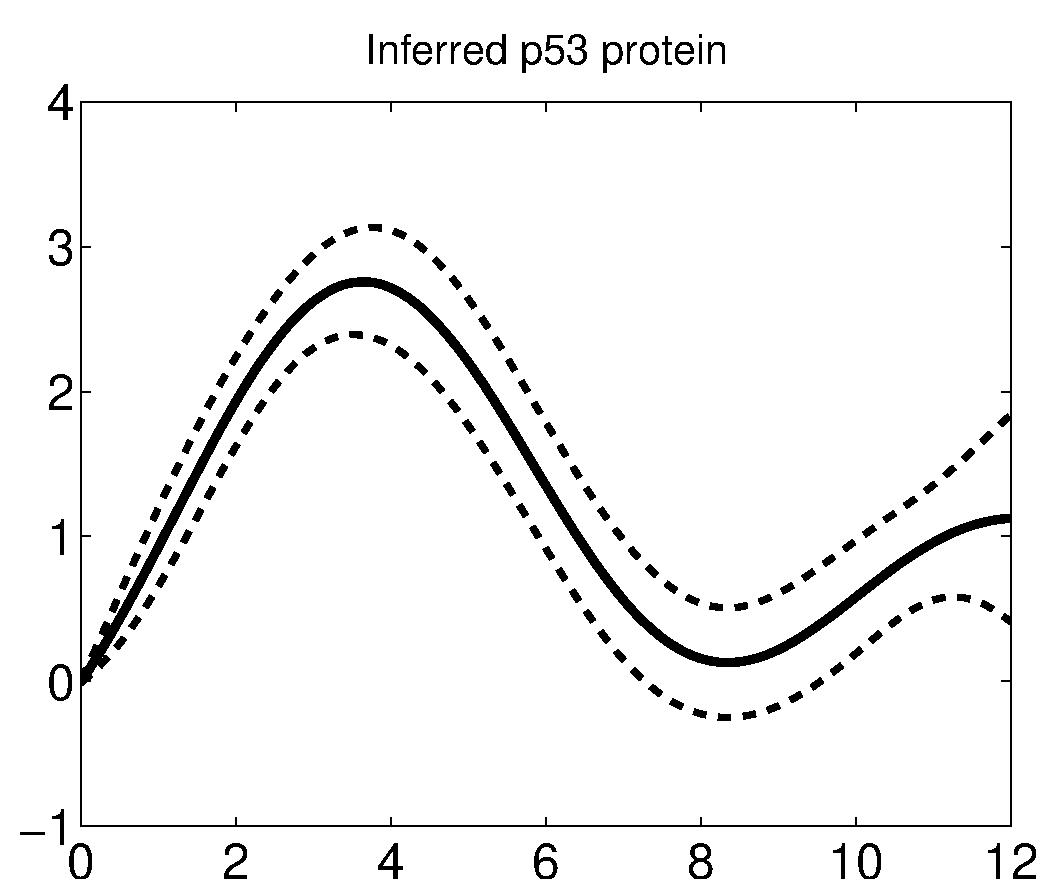
\includegraphics[height=1.4in, width=0.21\textwidth] {./diagrams/demBarenco1_profile3.eps} 	}
\subfigure[]{
	\label{fig:mlpact:b}
	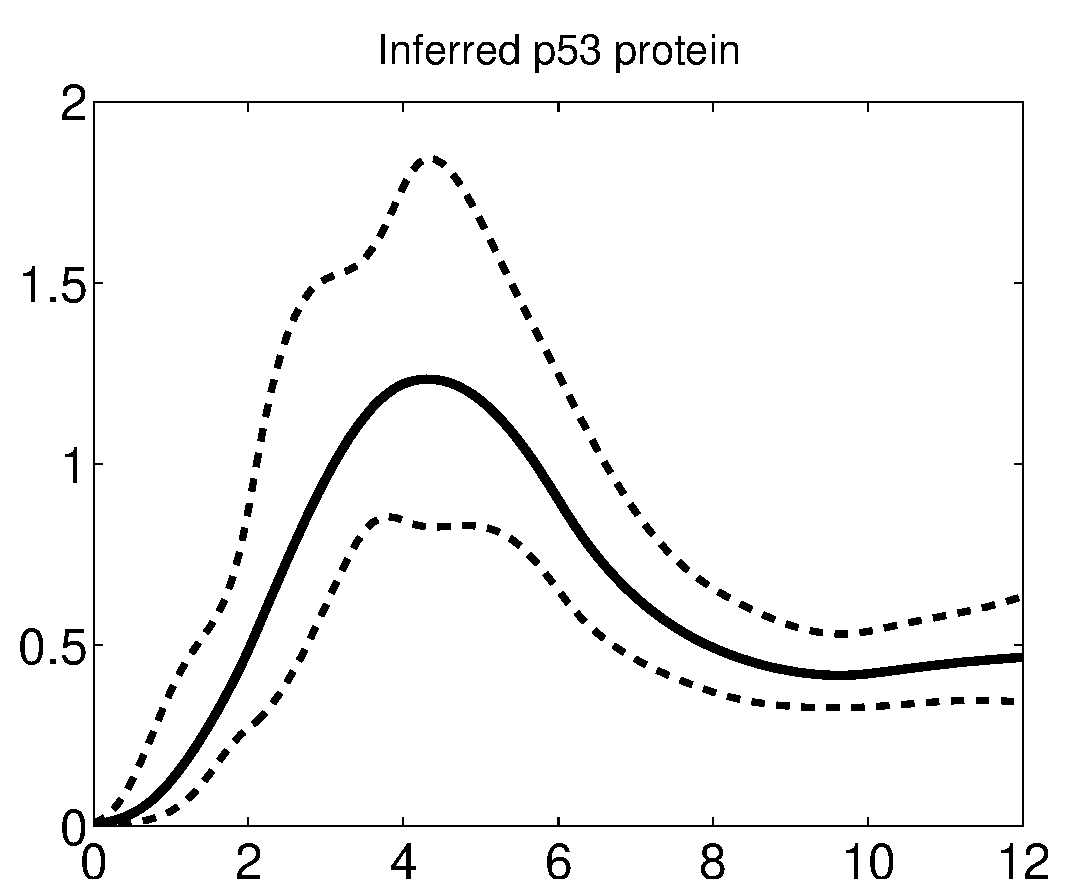
\includegraphics[height=1.4in, width=0.21\textwidth] {./diagrams/demBarencoMapMLPAct3_profile3.eps} }
\caption{Inferring p53 activity for a different replicate than
  Figure~\ref{fig:activation} (a) using the linear model; (b) using
  the nonlinear model with Michalis Menten kinetics and a positively
  constrained TF concentration.}
\label{fig:mlpact}
\end{figure}

\begin{figure*}[t]
\centering
\subfigure[]{
	\label{fig:repression:a}
	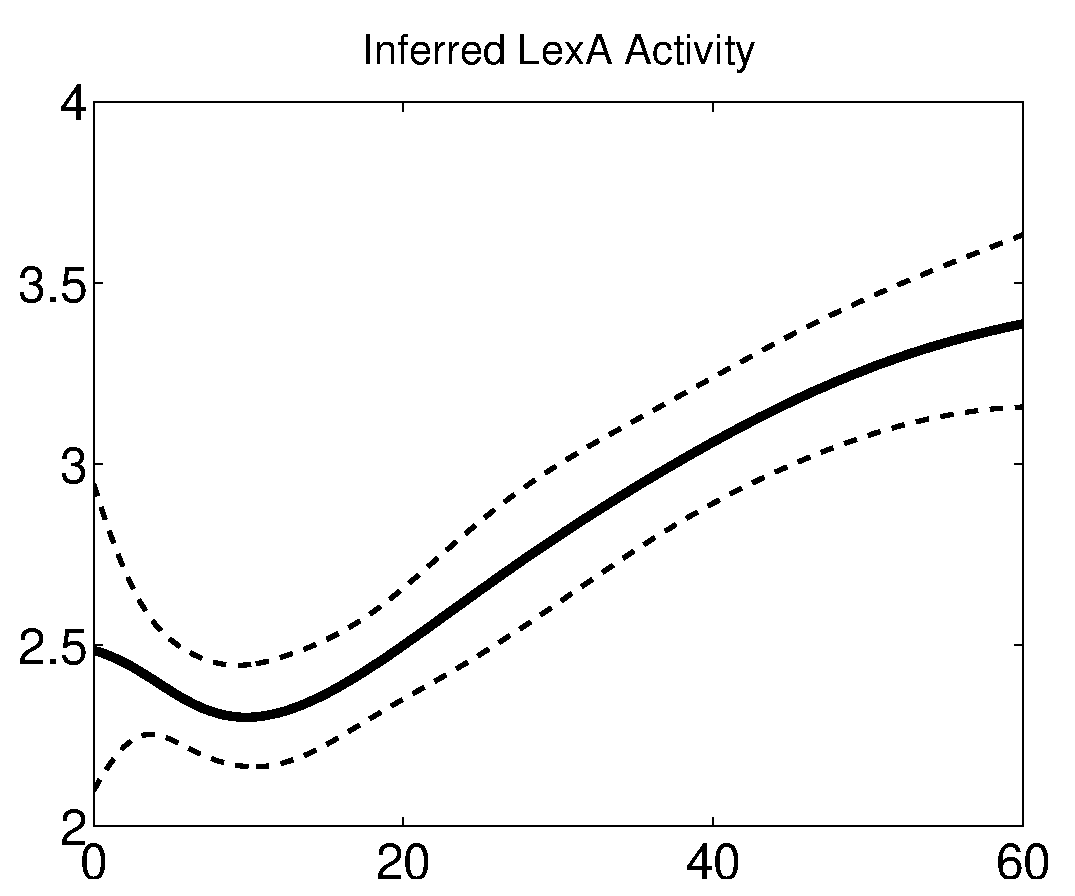
\includegraphics[height=1.6in, width=0.3\textwidth] {./diagrams/demMapFullEcoli_profile.eps} 	}
\subfigure[]{
	\label{fig:repression:b}
	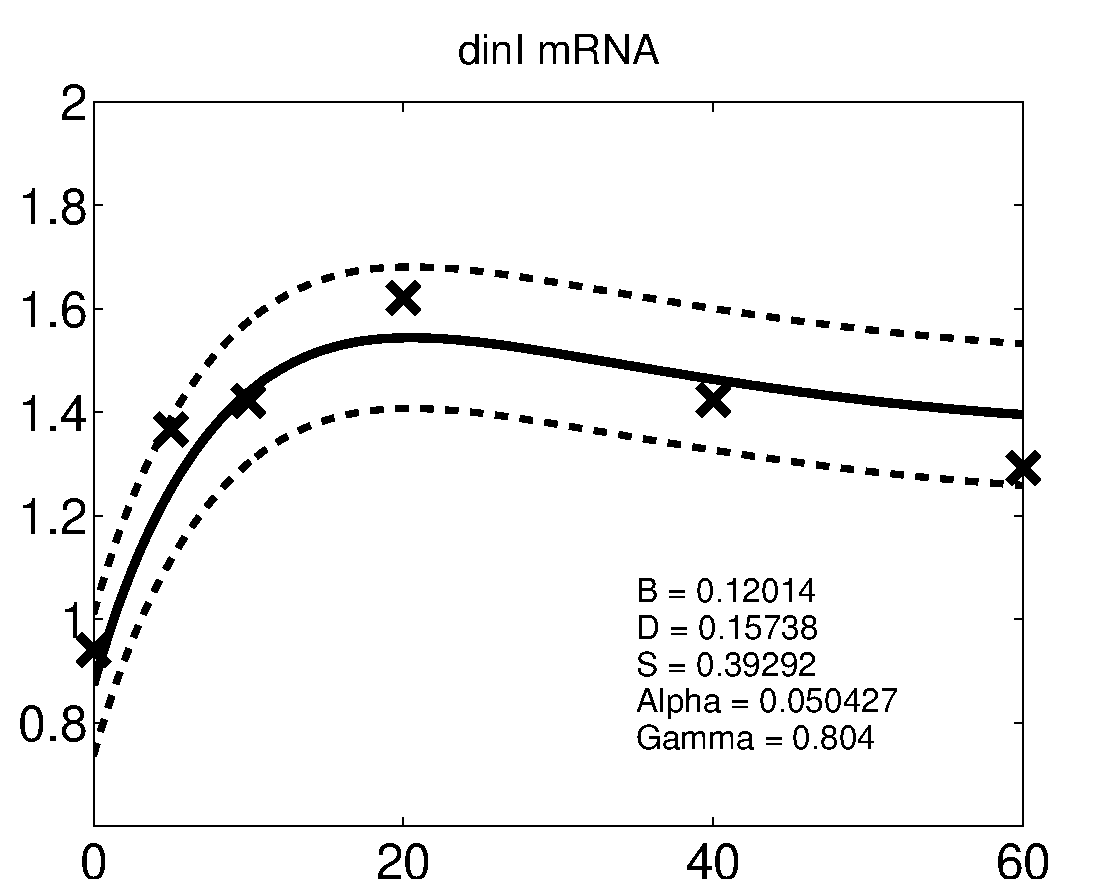
\includegraphics[height=1.6in, width=0.3\textwidth] {./diagrams/demMapFullEcoli_ExprsProfile_Rep1_Gene2.eps} }
\subfigure[]{
	\label{fig:repression:c}
	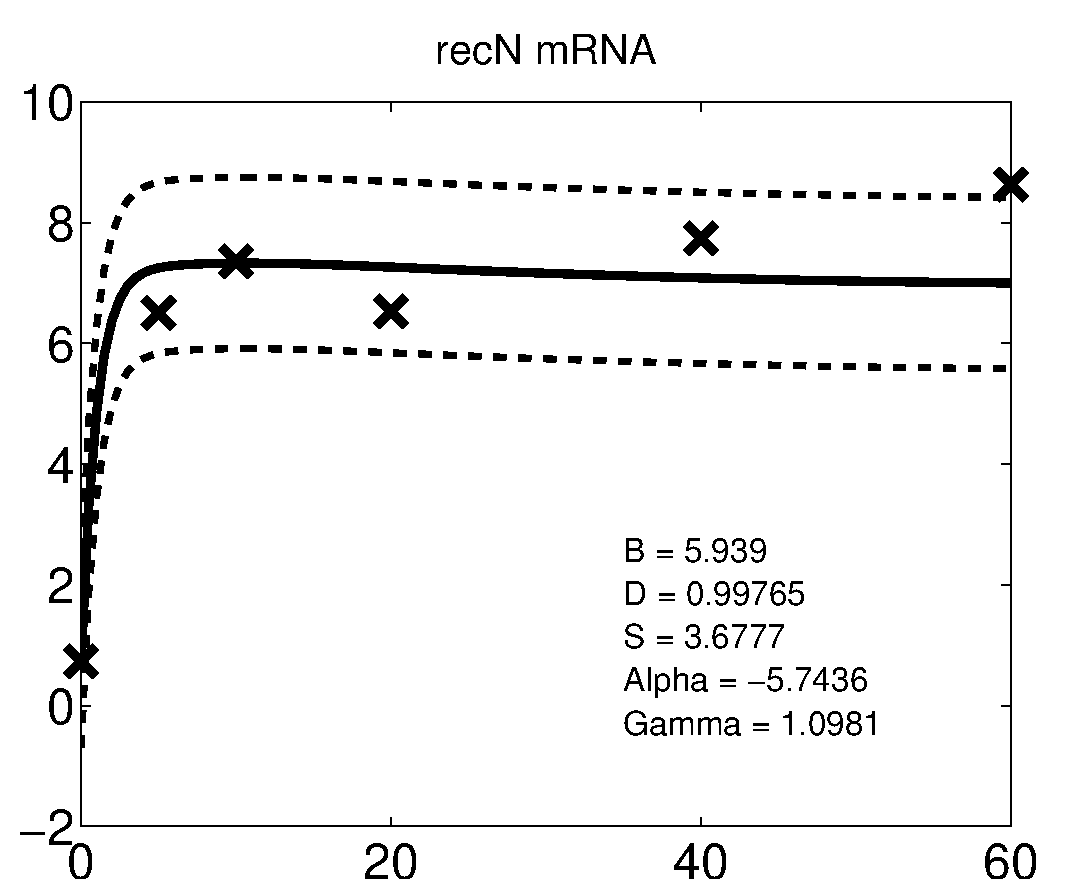
\includegraphics[height=1.6in, width=0.3\textwidth] {./diagrams/demMapFullEcoli_ExprsProfile_Rep1_Gene5.eps} }
\subfigure[]{
	\label{fig:repression:d}
	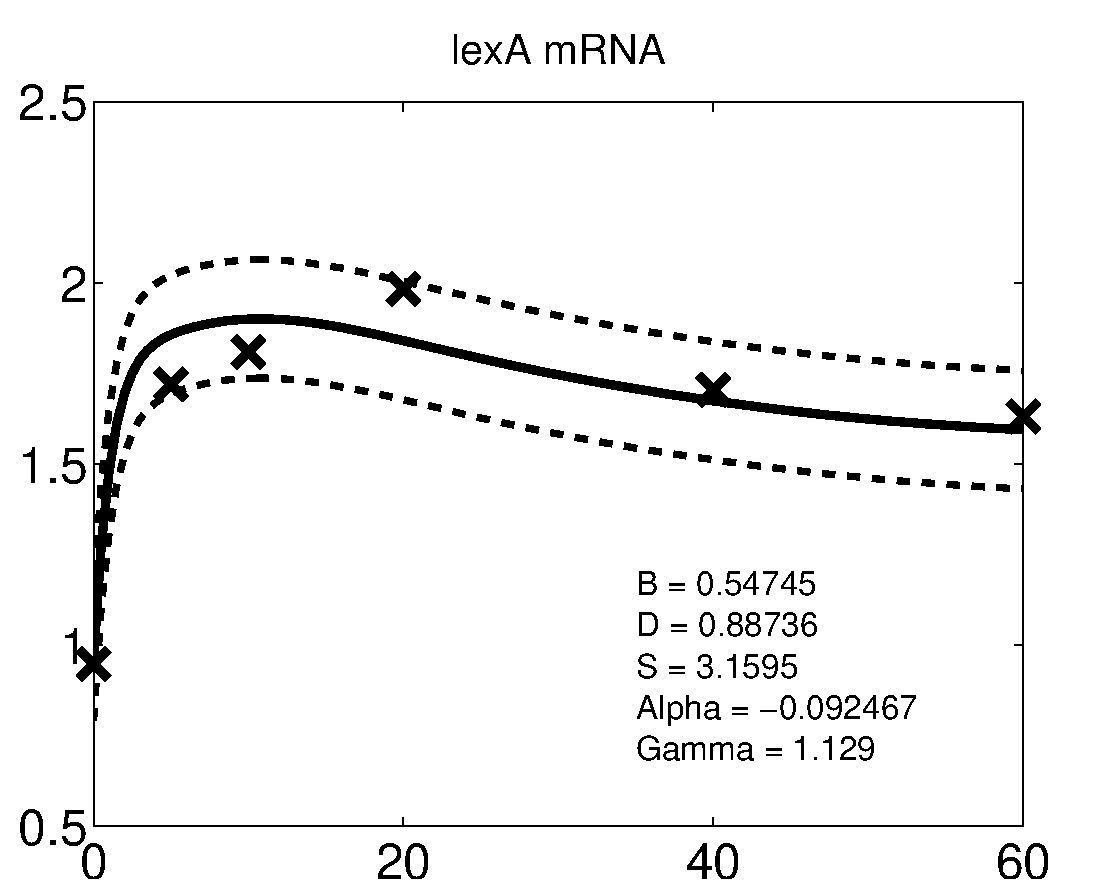
\includegraphics[height=1.6in, width=0.3\textwidth] {./diagrams/demMapFullEcoli_ExprsProfile_Rep1_Gene3.eps} }
\subfigure[]{
	\label{fig:repression:e}
	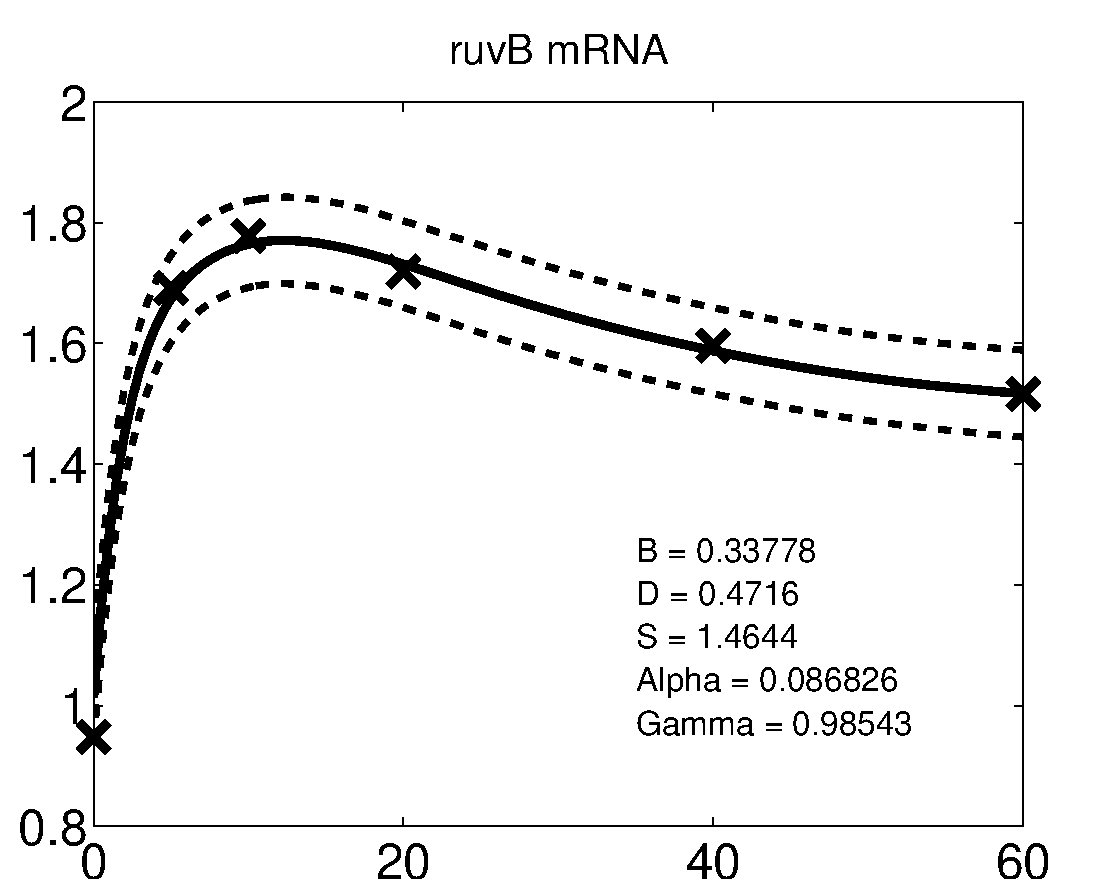
\includegraphics[height=1.6in, width=0.3\textwidth] {./diagrams/demMapFullEcoli_ExprsProfile_Rep1_Gene7.eps} }
\subfigure[]{
	\label{fig:repression:f}
	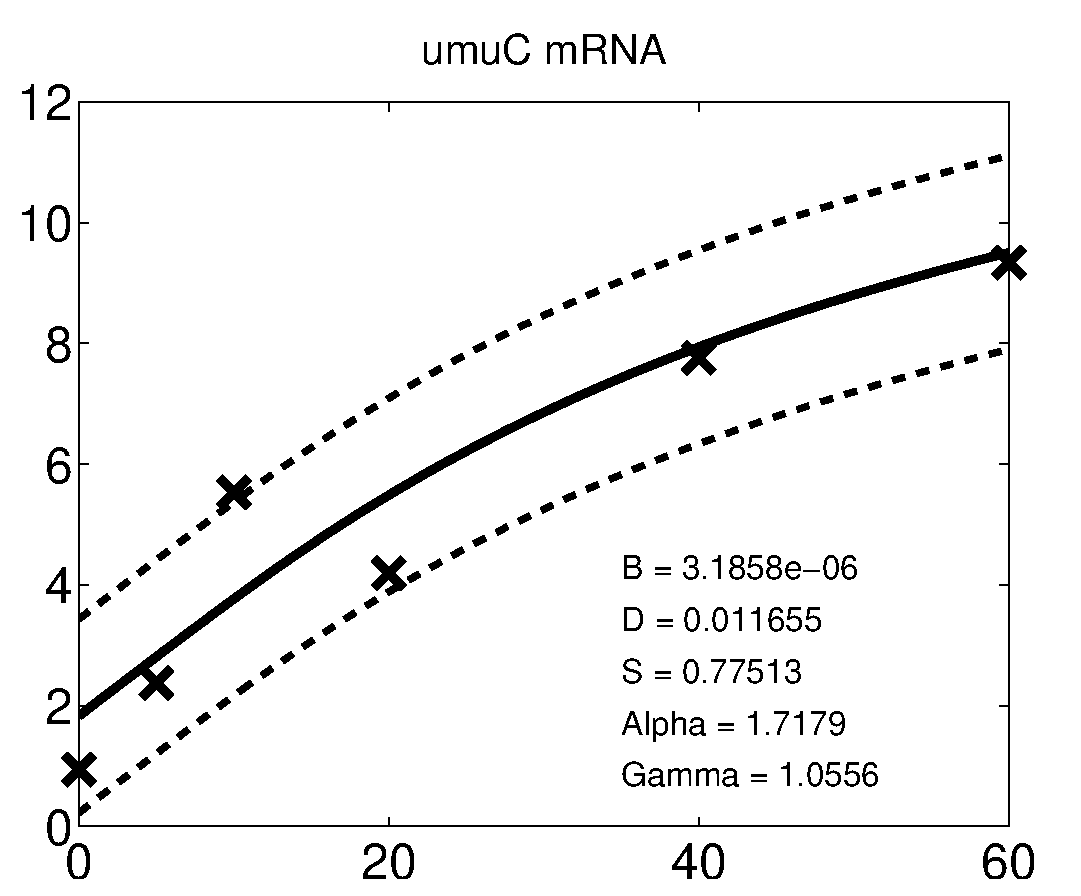
\includegraphics[height=1.6in, width=0.3\textwidth] {./diagrams/demMapFullEcoli_ExprsProfile_Rep1_Gene10.eps} }
\caption{Results for the repressor LexA. (a) predicted LexA
  concentration; (b) predicted expression level for dinI; (c)
  predicted expression level for recN; (d) predicted expression level
  for lexA; (e) predicted expression level for ruvB; (f) predicted
  expression level for umuC. Parameters shown were obtained by maximum
  likelihood. Standard errors were not available for this two-dye
  microarray data set and therefor a gene-specific noise variance
  parameter was estimated for each target gene.}
\label{fig:repression}
\end{figure*}

\subsubsection{Michaelis Menten Kinetics}

Michaelis Menten reaction kinetics were designed for the case where a
chemical reaction is enabled through an enzyme. If the concentration
of the enzyme is much lower than the concentration of the substrate
the reaction rate becomes limited by the reduced enzyme
availability. The justification in the context of modelling
transcription is that the reaction is that there are a limited number
of binding sites on the genome for the transcription factor. This
`bottle neck' has the same effect as a reduced availability of enzyme
and Michaelis Menten kinetics is therefore also appropriate as a model
of transcription.

We implemented Michaelis Menten kinetics for the p53 data by taking
the non-linearity to have the following form
%
\begin{equation}
g_j\left(f\left(t\right)\right)=\frac{e^{f\left(t\right)}}{\gamma_j + e^{f\left(t\right)}},
\end{equation}
%
where the Michaelis constant for the $i$th gene is given by $\gamma_i$
and we are using $f\left(t\right)$ to model the log of the TF
activity.

Figure~\ref{fig:mlpact}(b) shows the results of applying the above
kinetic model with positively constrained TF concentration to the p53
data set. It can be seen that the inferred distribution of TF profiles
no longer includes negative concentrations and the result is now
closer in shape to the replicate shown in Figure~\ref{fig:activation}.

\subsection{Repression\label{sub:repressionModel}}

The same framework can easily be adapted to the case of a repressor by
using an analogous Michaelis Menten model of repression,
%
\begin{equation}
g_j\left(f\left(t\right)\right)=\frac{1}{\gamma_j + e^{f\left(t\right)}},
\end{equation}
%
again using $f(t)$ to represent the log TF
concentration. \citet{Khanin:repression06} developed a method to infer
the TF profile and model parameters for this model. This involved a
coarse discretization of the TF profile, treating $f(t)$ as a
piecewise-constant function of time. They acknowledge that more
flexible parametric models for $f(t)$ will lead to an increase in the
number of parameters, which are therefore impossible to estimate by
maximum likelihood. Our approach avoids this explosion of parameters
by treating $f(t)$ as a functional parameter which is integrated out
before carrying out maximum likelihood for the other model parameters
(recall equation~(\ref{eqn:likelihood})).

We applied our method to the same microarray data as
\citet{Khanin:repression06}. They identify 14 target genes which are
repressed by the TF LexA in {\em E. Coli} and mRNA measurements for
these genes are collected over six time points. The amount of LexA is
reduced after UV irradiation, decreasing for a few minutes and then
recovering to its normal level.

In the case of repression we have to include the transient terms in
equation~(\ref{eq:linearSolution}),
\begin{equation}
x_{j}\left(t\right)=\alpha_je^{-D_{j}t}+\frac{B_{j}}{D_{j}}+S_{j}\int_{0}^{t}e^{-D_{j}\left(t-u\right)}g_j(f\left(u\right))\mathrm{d}u,\label{eq:linearSolutionRepressor}
\end{equation}
where $\{\alpha_j\}$ are an additional set of model parameters that have to
be inferred. 

The result for the inferred TF profile along with predictions for a
selection of target genes are shown in
Figure~\ref{fig:repression}. Our inferred TF profile and reconstructed
target gene profiles are similar to those obtained by
\citet{Khanin:repression06}, showing how different model parameters
can lead to very different target gene expression given the same
stimulous. However, whereas \citet{Khanin:repression06} had to use
interpolation to go from a discretized model to a continuous profile,
our GP representation avoids any need for discretization or
interpolation. The model parameters shown in the figure are estimated
by maximum likelihood.

\subsection{Cascaded Differential Equations\label{sub:cascadedDifferentialEquations}}

As a final example we consider a simple cascade of differential
equations.  Returning to the framework of the linear model we consider
the case where the TF protein is regulated at the level of
transcription.  In other words, we model the process of translation
from mRNA to protein for the TF, but we are only able to measure the
mRNA of the TF and of its targets. The simple model we consider would
only be appropriate in the case where the TF does not require
activation, \emph{e.g.} by phosphorolation, after translation. The
model is, therefore, not appropriate for many signalling pathways, but
seems sensible in the context of development where TFs are often
functional directly after translation.  We therefore considered an
example of the development of the mesoderm in \emph{Drosophila}
combining target gene predictions from ChIP-chip
data~\citep{Sandmann06} with microarray time-course data from
wild-type development~\citep{Tomancak02}.

We take the production rate of active transcription factor to be given by,
%
\begin{equation}
\frac{\mathrm{d}f\left(t\right)}{\mathrm{d}t}=\sigma y\left(t\right) - \delta f\left(t\right)
\end{equation}
%
where $\delta$ gives the decay rate of the active TF protein, $\sigma$
gives a rate of transcription and $y\left(t\right)$ is the
concentration of the transcription factor's mRNA. The solution for
$f(t)$, setting transient terms to zero, is
%
\begin{equation}
f(t) = \sigma \int_0^t y(v) \, \mathrm{e}^{\delta(v-t)} dv \ .
\end{equation}
%
If we assume that $y\left(t\right)$ was drawn from a GP with the
squared exponential covariance function, then $f\left(t\right)$ is
also a GP with the kernel being a special case of the one given by
equations~(\ref{eqn:kxjxj}) and (\ref{eqn:kxjf}). This gives us a new
covariance function governing $f\left(t\right)$. It turns out that we
can use this prior over $f\left(t\right)$ in the linear activation
model (equation~(\ref{eqn:linearModel})) and derive the associated
prior distribution for the target genes of the TF,
$\left\{x_{j}\left(t\right)\right\}_{j=1}^N$. The derivation and form
of the resulting covariance function are rather involved, but
remarkably all the integrals required can be calculated analytically
for the squared exponential covariance function given by
equation~(\ref{eqn:squaredExp}).

We applied the above driven input model to a simple cascade in
\emph{Drosophila} mesoderm development, focusing on the transcription
factor Mef2 (Myocyte enhancing factor 2). We selected six targets of
Mef2 identified by Chromatin immunoprecipitation (ChIP-chip)
assays~\citep{Sandmann06} and which were observed to be up-regulated
after Mef2 is expressed. Affymetrix time course microarray data from
wild-type embryos~\citep{Tomancak02} provides us with observations of
Mef2 expression ($y(t)$) and the expression of the target genes
${x_{j}\left(t\right)}$ at hourly intervals. The microarray time
course was replicated three times, and we used all three replicates to
fit the model parameters $\delta,\{B_j,D_j,S_j\}$ and the kernel
lengthscale $l$ by maximum likelihood (we set $\sigma=1$ without loss
of generality since the scale of the TF protein is arbitrarily
determined by the $S_j$ parameters).

Figure~\ref{fig:gpdisim} shows the results for one replicate. Error
bars associated with the mRNA data are obtained from the Affymetrix
probe-level processing of each replicate~\citep{Liu05}. In
Figure~\ref{fig:gpdisim}(a) we show the inferred mRNA profile for Mef2
along with the microarray data. In Figure~\ref{fig:gpdisim}(b) we show
the inferred TF profile for Mef2. Figures~\ref{fig:gpdisim}(c) and (d)
show the model predictions for two of the targets, along with the
associated expression data, showing again the difference in response
possible given different model parameters.

\begin{figure}
\centering
\subfigure[]{
	\label{fig:gpdisim:a}
	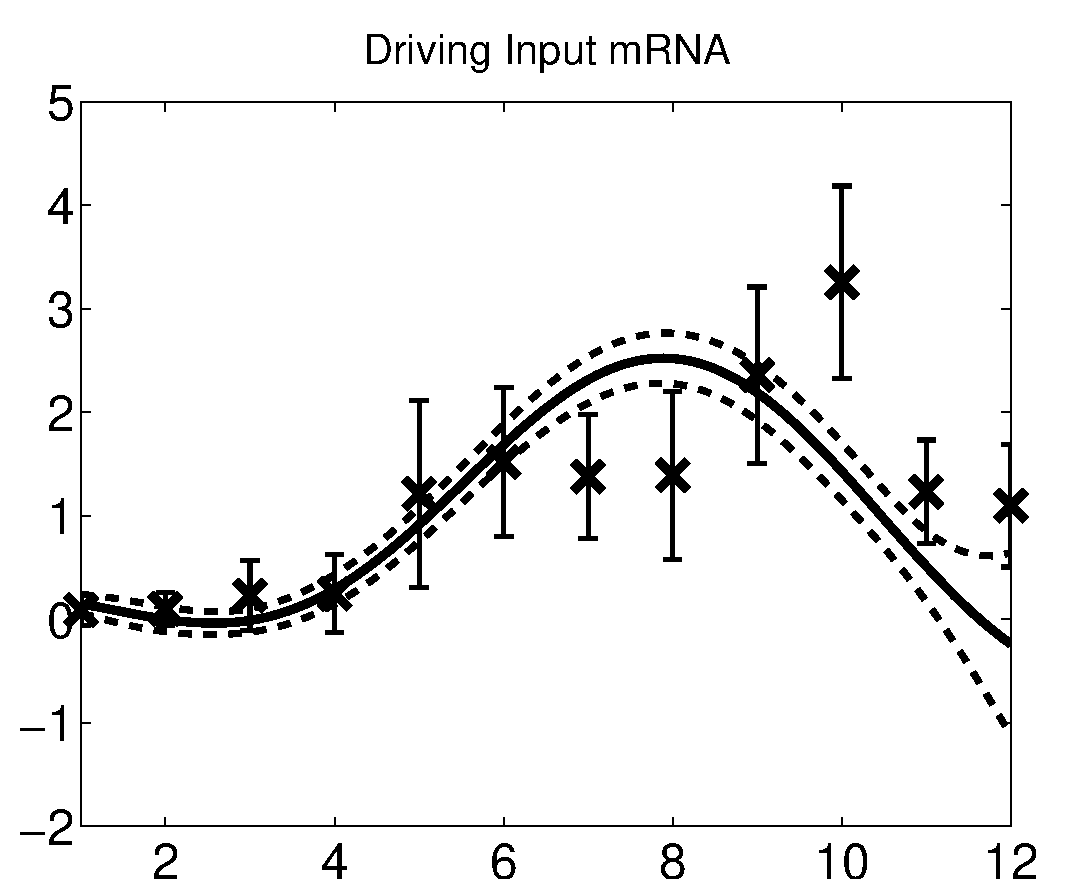
\includegraphics[height=1.4in, width=0.21\textwidth] {./diagrams/demMef2_ExprsProfile_Rep1_Gene1.eps} 	}
\subfigure[]{
	\label{fig:gpdisim:b}
	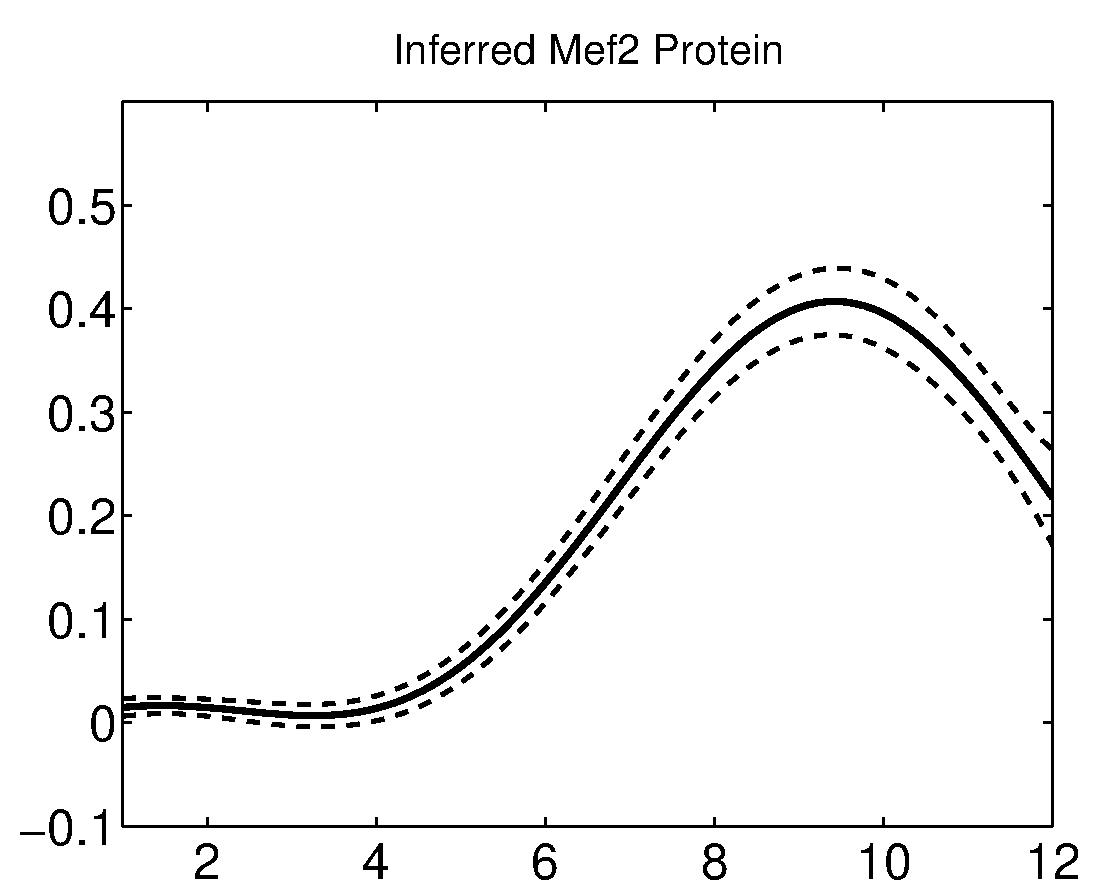
\includegraphics[height=1.4in, width=0.21\textwidth] {./diagrams/demMef2TF_profile_Rep1.eps} 	}
\subfigure[]{
	\label{fig:gpdisim:c}
	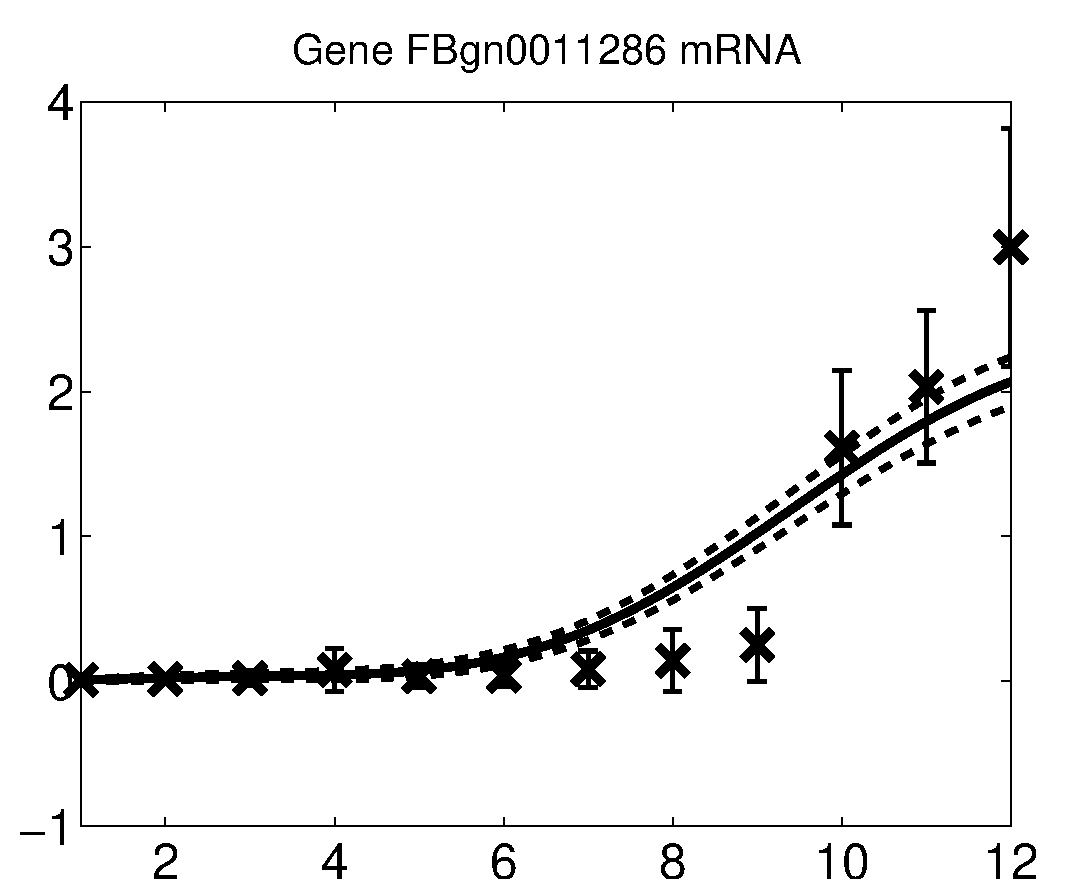
\includegraphics[height=1.4in, width=0.21\textwidth] {./diagrams/demMef2_ExprsProfile_Rep1_Gene2.eps} 	}
\subfigure[]{
	\label{fig:gpdisim:d}
	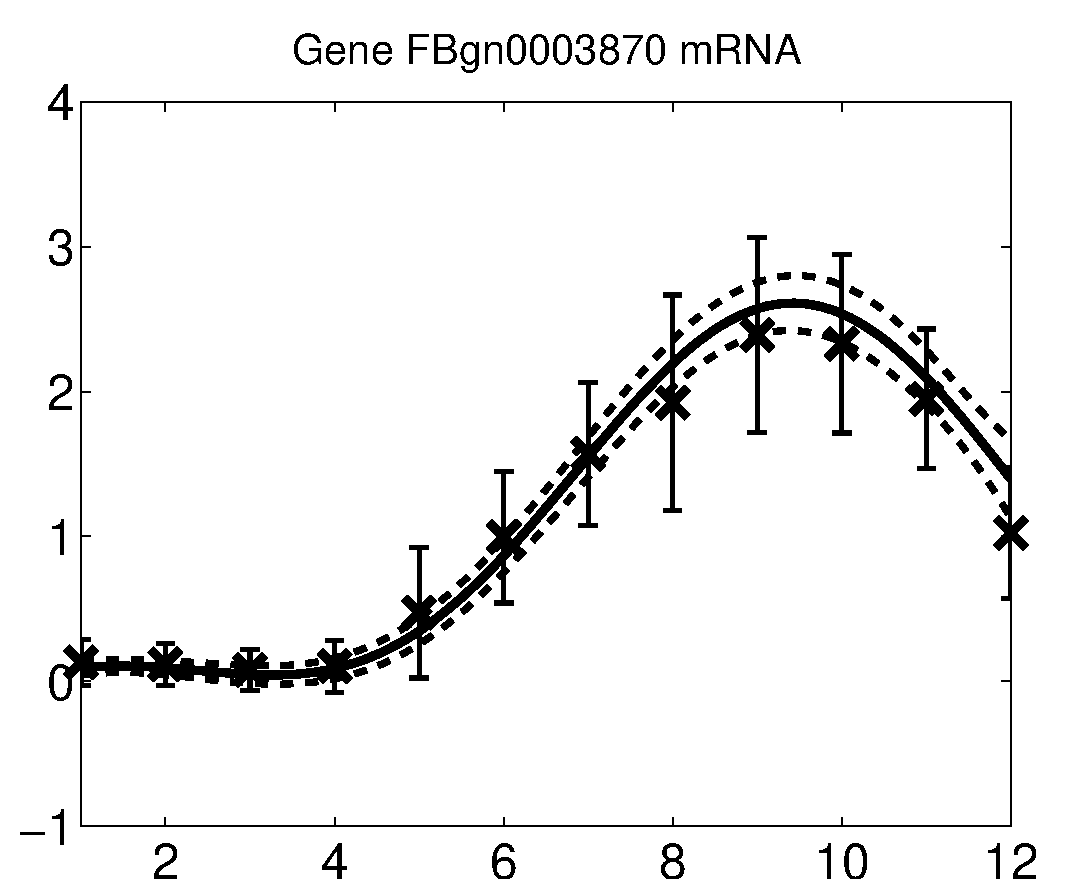
\includegraphics[height=1.4in, width=0.21\textwidth] {./diagrams/demMef2_ExprsProfile_Rep1_Gene4.eps} 	}
\caption{Results for Mef2 from one replicate: (a) Driving input mef2 mRNA
  concentration; (b) inferred Mef2 protein concentration; (c-d) reconstructed mRNA
  profiles of two example genes from the six used to train the
  model. Data points and error bars are obtained from probe-level
  analysis of the Affymetrix data using the puma package~\citep{Liu05}.}
\label{fig:gpdisim}
\end{figure}

We observe that using the TF mRNA data results in the model obtaining
tighter credibility intervals for the inferred TF. The fit to the
target gene expression looks reasonable, although the response in
Figure~\ref{fig:gpdisim}(c) appears to be sharper than predicted by
the model. It also appears that peak of the inferred Mef2 mRNA profile
precedes the peak in the data. The model here highlights the fact that
some of our simplifying assumptions are being violated by the
biology. The most critical assumption that we have made is that all of
the targets used to train the model are unique targets of Mef2. In
reality it is likely that other TFs are co-bound with Mef2. In future
work we expect to extend the model to account for these other TFs. We
are currently using unpublished ChIP-chip data (obtained from
E. Furlong, EMBL Heidelberg) for other TFs involved in mesoderm
development in order to refine our model and selection of targets.

\section{Discussion}

Gaussian processes allow for inference over chemical species
concentrations in a continuous time manner. In this paper, we have
laid out the basic technologies required for this inference and
highlighted some of the issues that arise: \emph{e.g.} dealing with
non linear response models and multiple interacting transcription
factors. \citeauthor{Barenco:ranked06} have already shown that these
models can be used for ranking targets of transcription factors. Such
rankings can also be given in the context of our models, both for
linear and non-linear response models.

Another important direction of future research will be scaling the
models used to much larger systems with multiple interacting
transcription factors. Larger systems will lead to an increase in
computational requirements, particularly if it is necessary to account
for correlations between multiple interacting latent chemical species.

The non-linear response models require particular approximations as
exact inference in these models is not tractable. One issue with the
Laplace approximation we have applied is that it is only responsive to
the mode of the posterior distribution. Variational approximations
\citep{Jordan:variational98} provide an alternative approach which can
lead to a rigorous lower bound on the likelihood. Finally, it also
makes sense to validate the quality of the approximation through
Markov chain Monte Carlo (MCMC) approximations. We are working towards
efficient MCMC algorithms for validating the quality of our
approximate inference.

All the experiments we have shown have been in the context of
transcription networks. However, the technologies are equally
applicable for other biological systems, such as metabolic networks.



\section*{Funding}

This work is funded by BBSRC Grant. No BBS/B/0076X {}``Improved
processing of microarray data with probabilistic models'', EPSRC
Grant. No EP/F005687/1 {}``Gaussian Process Models for Systems
Identification with Applications in Systems Biology'' and the EU FP6
Network of Excellence PASCAL.

\section*{Acknowledgement }

For data provision and assistance with our questions we would like to
thank Charles Girardot and Eileen Furlong of EMBL in Heidelberg
(mesoderm development in \emph{D. Melanogaster}), Martino Barenco and
Mike Hubank at the Institute of Child Health in UCL (p53 pathway) and
Raya Khanin and Ernst Wit of the University of Glasgow and the
University of Lancaster (\emph{E. coli} repressor system).

\bibliographystyle{plainnat}
\bibliography{toantti}


\end{document}
